\documentclass[tikz,border=3mm]{standalone}
\usepackage{tikz}

\begin{document}
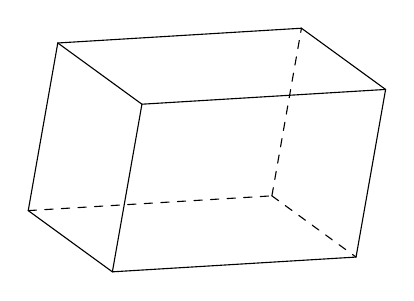
\begin{tikzpicture}[scale=1.15, line cap=round, line join=round]

% ================== 你主要改这里：尺寸与视角 ==================
\def\a{3.2}   % x 方向长度（底面宽）
\def\b{2.0}   % y 方向长度（底面深）
\def\c{1.8}   % z 方向长度（高度）

% 视角（单位：度）
\def\yaw{35}    % 绕 y 轴旋转（左右“转身”）
\def\pitch{20}  % 绕 x 轴旋转（上下“俯仰”）
\def\roll{-10}  % 绕 z 轴旋转（在纸面内再转一点，可设为 0）
% ============================================================

% 预计算三角函数
\pgfmathsetmacro{\cy}{cos(\yaw)}
\pgfmathsetmacro{\sy}{sin(\yaw)}
\pgfmathsetmacro{\cp}{cos(\pitch)}
\pgfmathsetmacro{\sp}{sin(\pitch)}
\pgfmathsetmacro{\cr}{cos(\roll)}
\pgfmathsetmacro{\sr}{sin(\roll)}

% -------- 面的可见性（1=朝向观察者，0=背向观察者）--------
% 这里假设投影是“丢弃 Z”，观察方向沿 +Z。
% 对长方体六个坐标面，法向分别是 ±x, ±y, ±z；
% 旋转后取法向的 Z 分量，Z>0 视为可见。
\pgfmathtruncatemacro{\fXp}{ifthenelse((- \sy*\cp) > 0,1,0)} % +x 面
\pgfmathtruncatemacro{\fXn}{ifthenelse((  \sy*\cp) > 0,1,0)} % -x 面
\pgfmathtruncatemacro{\fYp}{ifthenelse((  \sp)      > 0,1,0)} % +y 面
\pgfmathtruncatemacro{\fYn}{ifthenelse((- \sp)      > 0,1,0)} % -y 面
\pgfmathtruncatemacro{\fZp}{ifthenelse((  \cy*\cp)  > 0,1,0)} % +z 面
\pgfmathtruncatemacro{\fZn}{ifthenelse((- \cy*\cp)  > 0,1,0)} % -z 面

% -------- 8 个顶点：v0..v7（先在 3D，旋转后投影到 2D）--------
\foreach \i/\x/\y/\z in {
  0/0/0/0,
  1/\a/0/0,
  2/\a/\b/0,
  3/0/\b/0,
  4/0/0/\c,
  5/\a/0/\c,
  6/\a/\b/\c,
  7/0/\b/\c
}{
  % 绕 y 轴（yaw）
  \pgfmathsetmacro{\xone}{\x*\cy + \z*\sy}
  \pgfmathsetmacro{\yone}{\y}
  \pgfmathsetmacro{\zone}{-\x*\sy + \z*\cy}

  % 绕 x 轴（pitch）
  \pgfmathsetmacro{\xtwo}{\xone}
  \pgfmathsetmacro{\ytwo}{\yone*\cp - \zone*\sp}
  \pgfmathsetmacro{\ztwo}{\yone*\sp + \zone*\cp}

  % 绕 z 轴（roll，纸面内转一下）
  \pgfmathsetmacro{\X}{\xtwo*\cr - \ytwo*\sr}
  \pgfmathsetmacro{\Y}{\xtwo*\sr + \ytwo*\cr}

  \coordinate (v\i) at (\X,\Y);
}

% -------- 12 条棱：端点 u-v 以及相邻的两个面（用面可见性判断虚实）--------
\def\edgelist{
  0/1/\fYn/\fZn,
  1/2/\fXp/\fZn,
  2/3/\fYp/\fZn,
  3/0/\fXn/\fZn,
  4/5/\fYn/\fZp,
  5/6/\fXp/\fZp,
  6/7/\fYp/\fZp,
  7/4/\fXn/\fZp,
  0/4/\fXn/\fYn,
  1/5/\fXp/\fYn,
  2/6/\fXp/\fYp,
  3/7/\fXn/\fYp
}

% 先画隐藏棱（虚线），再画可见棱（实线）——这就是“遮掩顺序”
\foreach \u/\v/\fa/\fb in \edgelist{
  \pgfmathtruncatemacro{\vis}{ifthenelse((\fa+\fb)>0,1,0)}
  \ifnum\vis=0
    \draw[dashed] (v\u) -- (v\v);
  \fi
}
\foreach \u/\v/\fa/\fb in \edgelist{
  \pgfmathtruncatemacro{\vis}{ifthenelse((\fa+\fb)>0,1,0)}
  \ifnum\vis=1
    \draw (v\u) -- (v\v);
  \fi
}

\end{tikzpicture}
\end{document}
